\documentclass[10pt]{report}
\usepackage{a4wide}
\usepackage{epsfig}
\usepackage{array}
\usepackage{amsmath}
\usepackage{SIunits}
\usepackage{psfrag}
\usepackage{relsize}
\usepackage[section]{placeins}
\usepackage{listings}

\newif\ifpdf
\ifx\pdfoutput\undefined
  \pdffalse
\else
  \pdfoutput=1
  \pdftrue
\fi

\ifpdf
\pdfcompresslevel=9
\pdfinfo {
  /Title   (Qucs)
  /Subject (Technical Papers)
  /Author  (Stefan Jahn)
}
\fi

\makeatletter
\def\thickhrulefill{\leavevmode \leaders \hrule height 1pt\hfill \kern \z@}
\renewcommand{\maketitle}{\begin{titlepage}%
    \let\footnotesize\small
    \let\footnoterule\relax
    \parindent \z@
    \reset@font
    \null\vfil
    \vspace*{3cm}
    \begin{flushleft}
      \bf \huge \@title
    \end{flushleft}
    \par
    \hrule height 3pt
    \par
    \begin{flushright}
      \LARGE Technical Papers \par
    \end{flushright}
    \vskip 60\p@
    \vfill


    \begin{flushright}
      \Large \@author \par
    \end{flushright}

    \hrule height 3pt \par

\vspace*{24pt}

Copyright \copyright{} 2003, 2004 Michael Margraf 
\textless margraf@mwt.ee.tu-berlin.de\textgreater \par
Copyright \copyright{} 2003, 2004 Stefan Jahn 
\textless jahn@mwt.ee.tu-berlin.de\textgreater \par

\vspace*{12pt}

Permission is granted to copy, distribute and/or modify this document
under the terms of the GNU Free Documentation License, Version 1.1 or
any later version published by the Free Software Foundation.  A copy
of the license is included in the section entitled "GNU Free
Documentation License".

\vspace*{1cm}

  \end{titlepage}%
  \setcounter{footnote}{0}%
}
\makeatother

\author{Michael Margraf \\ Stefan Jahn}
\title{Qucs}
\date{}

\begin{document}

\maketitle

\tableofcontents

\setlength{\parindent}{0pt}
\newpage

\chapter*{Mathematical expressions and conversions}
\addcontentsline{toc}{chapter}{Mathematical expressions and conversions}

\section*{Scattering parameters}
\addcontentsline{toc}{section}{Scattering parameters}

\subsection*{Recalculating $\mathbf{50\ohm}$-S-parameters for arbitrary port impedances}
\addcontentsline{toc}{subsection}{Recalculating $50\ohm$-S-parameters for arbitrary port impedances}

During S-parameter simulation it is necessary to have all components
in a circuit normalized to the same impedance.  In the field of high
frequency techniques this is usually $50\ohm$.  In order to allow port
impedances other than $50\ohm$ in a simulation the following two step
process must be applied to the resulting S-parameter analysis.

\begin{equation}
\left[\underline{N}\right] = 
\left(\left[\underline{S}\right] - \left[\underline{R}\right]\right) \cdot
\left(\left[\underline{E}\right] - \left[\underline{R}\right] \cdot \left[\underline{S}\right]\right)^{-1}
\end{equation}

\begin{equation}
\underline{N}_{nm} = \underline{S}_{nm}\cdot \sqrt{\dfrac{Z^{m}}{Z^{n}}}\cdot
\dfrac{Z^{n} + Z_{0}}{Z^{m} + Z_{0}}
\end{equation}

With

\addvspace{12pt}

\begin{tabular}{rll}
$Z_{0}$ & = & $50\ohm$\\& &\\
$\left[\underline{E}\right]$ & = &
$\begin{pmatrix}
1 & 0 & \ldots & 0\\
0 & 1 & \ldots & 0\\
\vdots & \vdots & \ddots & \vdots\\
0 & 0 & \ldots & 1\\
\end{pmatrix}$
identity matrix\\& &\\
$\left[\underline{S}\right]$ & = & original $50\ohm$-S-parameter matrix\\& &\\
$\left[\underline{N}\right]$ & = & recalculated scattering matrix\\& &\\
$\left[\underline{R}\right]$ & = &
$\begin{pmatrix}
\underline{r}(Z_{1}) & 0 & \ldots & 0\\
0 & \underline{r}(Z_{2}) & \ldots & 0\\
\vdots & \vdots & \ddots & \vdots\\
0 & 0 & \ldots & \underline{r}(Z_{n})\\
\end{pmatrix}$
reflection coefficient matrix\\& &\\
$\underline{r}(Z_{n})$ & = &
$\dfrac{Z_{n} - Z_{0}}{Z_{n} + Z_{0}}$
reflection coefficient of impedance at port n\\& &\\
\end{tabular}

And furthermore

\addvspace{12pt}

\begin{tabular}{rll}
$\left[\underline{X}\right]^{-1}$ & = & 
inverted matrix of $\left[\underline{X}\right]$\\& &\\
$\underline{X}_{nm}$ & = & 
element of matrix $\left[\underline{X}\right]$ at row n and column m\\& &\\
\end{tabular}

\subsection*{Differential S-parameter ports}
\addcontentsline{toc}{subsection}{Differential S-parameter ports}

The implemented algorithm for the S-parameter analysis calculates
S-parameters in terms of the ground node.  In order to allow
differential S-parameters as well it is necessary to insert an ideal
impedance transformer with a turns ratio of 1:1 between the
differential port and the device under test.

\begin{figure}[ht]
\begin{center}
\includegraphics[width=12cm]{differential}
\end{center}
\caption{transformation of differential port into single ended port}
\label{fig:differential}
\end{figure}
\FloatBarrier

The S-parameter matrix of the inserted ideal transformer being a three
port device can be written as follows.

\begin{equation}
\begin{pmatrix}
S
\end{pmatrix}
= \dfrac{1}{3}\cdot
\begin{pmatrix}
1 & 2 & -2\\
2 & 1 & 2\\
-2 & 2 & 1\\
\end{pmatrix}
\end{equation}

This transformation can be applied to each S-parameter port in a
circuit regardless whether it is actually differential or not.

\addvspace{12pt}

It is also possible to do the impedance transformation within this step
(for S-parameter ports with impedances different than $50\ohm$). This can
be done by using a transformer with an impedance ration of

\begin{equation}
r=T^2=\frac{50\ohm}{Z}
\end{equation}

With $Z$ being the S-parameter port impedance. The S-parameter matrix of
the inserted ideal transformer now writes as follows.

\begin{equation}
\begin{pmatrix}
S
\end{pmatrix}
= \dfrac{1}{2\cdot Z_0+Z}\cdot
\begin{pmatrix}
2\cdot Z_0-Z              & 2\cdot\sqrt{Z_0\cdot Z}  & -2\cdot\sqrt{Z_0\cdot Z}\\
2\cdot\sqrt{Z_0\cdot Z}   & Z                        & 2\cdot Z_0\\
-2\cdot\sqrt{Z_0\cdot Z}  & 2\cdot Z_0               & Z\\
\end{pmatrix}
\end{equation}

With $Z$ being the new S-parameter port impedance and $Z_0$ being $50\ohm$.

\section*{Scattering parameters of components}
\addcontentsline{toc}{section}{Scattering parameters of components}

\subsection*{Resistor}
\addcontentsline{toc}{subsection}{Resistor}

The scattering parameters of an ideal, ohmic resistor with resistance
$R$ writes as follows.

\begin{equation}
S_{11} = S_{22} = \frac{R}{2\cdot Z_0+R} \\
\end{equation}
\begin{equation}
S_{12} = S_{21} = 1-S_{11} = \frac{2\cdot Z_0}{2\cdot Z_0+R}
\end{equation}

\subsection*{Capacitor}
\addcontentsline{toc}{subsection}{Capacitor}

The scattering parameters of an ideal capacitor with capacitance $C$
writes as follows.

\begin{equation}
S_{11} = S_{22} = \frac{1}{2\cdot Z_0\cdot j\omega C+1} \\
\end{equation}
\begin{equation}
S_{12} = S_{21} = 1-S_{11}
\end{equation}

\subsection*{Inductor}
\addcontentsline{toc}{subsection}{Inductor}

The scattering parameters of an ideal inductor with inductance $L$
writes as follows.

\begin{equation}
S_{11} = S_{22} = \frac{j\omega L}{2\cdot Z_0 + j\omega L} \\
\end{equation}
\begin{equation}
S_{12} = S_{21} = 1-S_{11}
\end{equation}

\subsection*{DC Block}
\addcontentsline{toc}{subsection}{DC Block}

A DC block is a capacitor with an infinite capacitance.  The
scattering parameters, therefore, writes as follows.

\begin{equation}
\begin{pmatrix}
S
\end{pmatrix}
=
\begin{pmatrix}
0 & 1\\
1 & 0\\
\end{pmatrix}
\end{equation}

\subsection*{DC Feed}
\addcontentsline{toc}{subsection}{DC Feed}

A DC feed is an inductor with an infinite inductance.  The scattering
parameters, therefore, writes as follows.

\begin{equation}
\begin{pmatrix}
S
\end{pmatrix}
=
\begin{pmatrix}
1 & 0\\
0 & 1\\
\end{pmatrix}
\end{equation}

\subsection*{Bias T}
\addcontentsline{toc}{subsection}{Bias T}

A bias T is a combination of a DC block and a DC feed
(fig. \ref{fig:biast}).  The scattering parameters, therefore, writes
as follows.

\begin{equation}
\begin{pmatrix}
S
\end{pmatrix}
=
\begin{pmatrix}
0 & 1 & 0\\
1 & 0 & 0\\
0 & 0 & 1\\
\end{pmatrix}
\end{equation}

\begin{figure}[ht]
\begin{center}
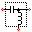
\includegraphics[width=3.5cm]{biast}
\end{center}
\caption{bias t}
\label{fig:biast}
\end{figure}
\FloatBarrier

\subsection*{Transformer}
\addcontentsline{toc}{subsection}{Transformer}

Using the port numbers depicted in fig. \ref{fig:trafo}, the
scattering parameters of an ideal transformer with voltage
transformation ratio $T$ (number of turns) writes as follows.

\begin{equation}
S_{14} = S_{22} = S_{33} = S_{41} = \frac{1}{T^2+1}
\end{equation}
\begin{equation}
S_{12} = -S_{13} = S_{21} = -S_{24} = -S_{31} = S_{34} = -S_{42} = S_{43} = T\cdot S_{22}
\end{equation}
\begin{equation}
S_{11} = S_{23} = S_{32} = S_{44} = T\cdot S_{12}
\end{equation}

\begin{figure}[ht]
\begin{center}
\includegraphics[width=4cm]{trafo}
\end{center}
\caption{transformer}
\label{fig:trafo}
\end{figure}
\FloatBarrier

\subsection*{Symmetrical transformer}
\addcontentsline{toc}{subsection}{Symmetrical transformer}

Using the port numbers depicted in fig. \ref{fig:symtrafo}, the
scattering parameters of an ideal, symmetrical transformer with
voltage transformation ratio (number of turns) $T_1$ and $T_2$,
respectively, writes as follows.

\begin{equation}
denom = T_1^2+T_2^2+T_1^2\cdot T_2^2
\end{equation}
\begin{eqnarray}
S_{11} = S_{66} = \frac{T_2^2}{denom}  &  \qquad S_{16} = S_{61} = 1-S_{11} \\
S_{44} = S_{55} = \frac{T_1^2}{denom}  &  \qquad S_{45} = S_{54} = 1-S_{44} \\
S_{22} = S_{33} = \frac{T_1^2\cdot T_2^2}{denom}  &  \qquad S_{23} = S_{32} = 1-S_{22} \\
\end{eqnarray}
\begin{equation}
S_{12} = S_{21} = -S_{13} = -S_{31} = -S_{26} = -S_{62} = S_{36} = S_{63}
       = \frac{T_1\cdot T_2^2}{denom}
\end{equation}
\begin{equation}
-S_{24} = -S_{42} = S_{25} = S_{52} = S_{34} = S_{43} = -S_{35} = -S_{53}
       = \frac{T_1^2\cdot T_2}{denom}
\end{equation}
\begin{equation}
-S_{14} = -S_{41} = S_{15} = S_{51} = S_{46} = S_{64} = -S_{56} = -S_{65}
       = \frac{T_1\cdot T_2}{denom}
\end{equation}

\begin{figure}[ht]
\begin{center}
\includegraphics[width=4cm]{symtrafo}
\end{center}
\caption{symmetrical transformer}
\label{fig:symtrafo}
\end{figure}
\FloatBarrier

\subsection*{Attenuator}
\addcontentsline{toc}{subsection}{Attenuator}

The scattering parameters of an ideal attenuator with attenuation $L$
(loss) (or gain $G=1/L$) in reference to the impedance $Z_{ref}$ writes as follows.

\begin{equation}
r = \frac{Z_0-Z_{ref}}{Z_0+Z_{ref}}
\end{equation}
\begin{equation}
S_{11} = S_{22} = \frac{r\cdot(1-G^2)}{G^2-r^2} = \frac{r\cdot(L^2-1)}{1-r^2\cdot L^2}
\end{equation}
\begin{equation}
S_{12} = S_{21} = \frac{G\cdot(1-r^2)}{G^2-r^2} = \frac{L\cdot(1-r^2)}{1-r^2\cdot L^2}
\end{equation}

\subsection*{Isolator}
\addcontentsline{toc}{subsection}{Isolator}

An isolator is a one-way two-port, transporting incoming waves
lossless from the input (port 1) to the output (port 2), but consuming
all waves flowing into the output. With the reference impedance of the
input $Z_1$ and the one of the output $Z_2$, the scattering parameters
of an ideal isolator writes as follows.

\begin{equation}
S_{11} = \frac{Z_1-Z_0}{Z_1+Z_0}
\end{equation}
\begin{equation}
S_{12} = 0
\end{equation}
\begin{equation}
S_{22} = \frac{Z_2-Z_0}{Z_2+Z_0}
\end{equation}
\begin{equation}
S_{21} = \sqrt{1-(S_{11})^2}\cdot\sqrt{1-(S_{22})^2}
\end{equation}

\subsection*{Circulator}
\addcontentsline{toc}{subsection}{Circulator}

A circulator is a 3-port device, transporting incoming waves lossless
from port 1 to port 2, from port 2 to port 3 and from port 3 to port
1.  In all other directions, there is no energy flow.  With the
reference impedances $Z_1$, $Z_2$ and $Z_3$ for the ports 1, 2 and 3
the scattering matrix of an ideal circulator writes as follows.

\begin{equation}
denom = 1-r_1\cdot r_2\cdot r_3
\end{equation}
\begin{equation}
r_1 = \frac{Z_0-Z_1}{Z_0+Z_1} \qquad,\qquad 
r_2 = \frac{Z_0-Z_2}{Z_0+Z_2} \qquad,\qquad 
r_3 = \frac{Z_0-Z_3}{Z_0+Z_3}
\end{equation}
\begin{equation}
S_{11} = \frac{r_2\cdot r_3 - r_1}{denom} \qquad,\qquad 
S_{22} = \frac{r_1\cdot r_3 - r_2}{denom} \qquad,\qquad 
S_{33} = \frac{r_1\cdot r_2 - r_3}{denom}
\end{equation}
\begin{equation}
S_{12} = \sqrt{\frac{Z_2}{Z_1}}\cdot\frac{Z_1+Z_0}{Z_2+Z_0}\cdot\frac{r_3\cdot(1-r_1^2)}{denom}
\qquad,\qquad 
S_{13} = \sqrt{\frac{Z_3}{Z_1}}\cdot\frac{Z_1+Z_0}{Z_3+Z_0}\cdot\frac{1-r_1^2}{denom}
\end{equation}
\begin{equation}
S_{21} = \sqrt{\frac{Z_1}{Z_2}}\cdot\frac{Z_2+Z_0}{Z_1+Z_0}\cdot\frac{1-r_2^2}{denom}
\qquad,\qquad 
S_{23} = \sqrt{\frac{Z_3}{Z_2}}\cdot\frac{Z_2+Z_0}{Z_3+Z_0}\cdot\frac{r_1\cdot(1-r_2^2)}{denom}
\end{equation}
\begin{equation}
S_{31} = \sqrt{\frac{Z_1}{Z_3}}\cdot\frac{Z_3+Z_0}{Z_1+Z_0}\cdot\frac{r_2\cdot(1-r_3^2)}{denom}
\qquad,\qquad 
S_{32} = \sqrt{\frac{Z_2}{Z_3}}\cdot\frac{Z_3+Z_0}{Z_2+Z_0}\cdot\frac{1-r_3^2}{denom}
\end{equation}

\subsection*{Phase shifter}
\addcontentsline{toc}{subsection}{Phase shifter}

The scattering parameters of an ideal phase shifter with phase shift
$\phi$ and reference impedance $Z_{ref}$ writes as follows.

\begin{equation}
r = \frac{Z_0-Z_{ref}}{Z_0+Z_{ref}}
\end{equation}
\begin{equation}
S_{11} = S_{22} = \frac{r\cdot\left(\exp(j\cdot 2\phi)-1\right)}{1-r^2\cdot\exp(j\cdot 2\phi)}
\end{equation}
\begin{equation}
S_{12} = S_{21} = \frac{(1-r^2)\cdot\exp(j\cdot\phi)}{1-r^2\cdot\exp(j\cdot 2\phi)}
\end{equation}


\subsection*{Gyrator}
\addcontentsline{toc}{subsection}{Gyrator}

A gyrator is an impedance inverter.  Thus, for example, it converts a
capacitance into an inductance and vice versa.  The scattering matrix
of an ideal gyrator with the ratio $R$ writes as follows.

\begin{equation}
r = \frac{R}{Z_{ref}} = \frac{1}{G\cdot Z_{ref}}
\end{equation}
\begin{equation}
S_{11} = S_{22} = S_{33} = S_{44} = \frac{R^2}{4\cdot Z_{ref}^2 + R^2} = \frac{r^2}{r^2+4}
\end{equation}
\begin{equation}
S_{14} = S_{23} = S_{32} = S_{41} = 1-S_{11}
\end{equation}
\begin{equation}
S_{12} = -S_{13} = -S_{21} = S_{24} = S_{31} = -S_{34} = -S_{42} = S_{43} = \frac{2\cdot r}{r^2+4}
\end{equation}

\subsection*{Voltage and current sources}
\addcontentsline{toc}{subsection}{Voltage and current sources}

All voltage sources (AC and DC) are short circuits and therefore their
S-parameter matrix equals the one of the DC block.  All current
sources are open circuits and therefore their S-parameter matrix
equals the one of the DC feed.

\subsection*{Controlled voltage and current sources}
\addcontentsline{toc}{subsection}{Controlled voltage and current sources}

The scattering matrix of the voltage controlled current source
depicted in fig. \ref{fig:xCCS} (left) writes as follows ($\tau$ is
time delay).

\begin{equation}
S_{11} = S_{22} = S_{33} = S_{44} = 1
\end{equation}
\begin{equation}
S_{12} = S_{13} = S_{14} = S_{23} = S_{32} = S_{41} = S_{42} = S_{43} = 0
\end{equation}
\begin{equation}
S_{21} = S_{34} = 2\cdot G\cdot \exp(j\pi-j\omega\tau)
\end{equation}
\begin{equation}
S_{24} = S_{31} = 2\cdot G\cdot \exp(-j\omega\tau)
\end{equation}

\begin{figure}[ht]
\begin{center}
\includegraphics[width=8cm]{xCCS}
\end{center}
\caption{voltage controlled current source (left) and current controlled current source (right)}
\label{fig:xCCS}
\end{figure}
\FloatBarrier

The scattering matrix of the current controlled current source
depicted in fig. \ref{fig:xCCS} (right) writes as follows ($\tau$ is
time delay).

\begin{equation}
S_{14} = S_{22} = S_{33} = S_{41} = 1
\end{equation}
\begin{equation}
S_{11} = S_{12} = S_{13} = S_{23} = S_{32} = S_{42} = S_{43} = S_{44} = 0
\end{equation}
\begin{equation}
S_{21} = S_{34} = G\cdot \exp(j\pi-j\omega\tau)
\end{equation}
\begin{equation}
S_{24} = S_{31} = G\cdot \exp(-j\omega\tau)
\end{equation}

The scattering matrix of the voltage controlled voltage source
depicted in fig. \ref{fig:xCVS} (left) writes as follows ($\tau$ is
time delay).

\begin{equation}
S_{11} = S_{23} = S_{32} = S_{44} = 1
\end{equation}
\begin{equation}
S_{12} = S_{13} = S_{14} = S_{22} = S_{33} = S_{41} = S_{42} = S_{43} = 0
\end{equation}
\begin{equation}
S_{21} = S_{34} = G\cdot \exp(-j\omega\tau)
\end{equation}
\begin{equation}
S_{24} = S_{31} = G\cdot \exp(j\pi-j\omega\tau)
\end{equation}

\begin{figure}[ht]
\begin{center}
\includegraphics[width=8cm]{xCVS}
\end{center}
\caption{voltage controlled voltage source (left) and current controlled voltage source (right)}
\label{fig:xCVS}
\end{figure}
\FloatBarrier

The scattering matrix of the current controlled voltage source
depicted in fig. \ref{fig:xCVS} (right) writes as follows ($\tau$ is
time delay).

\begin{equation}
S_{14} = S_{23} = S_{32} = S_{41} = 1
\end{equation}
\begin{equation}
S_{11} = S_{12} = S_{13} = S_{22} = S_{33} = S_{42} = S_{43} = S_{44} = 0
\end{equation}
\begin{equation}
S_{21} = S_{34} = \frac{G}{2}\cdot \exp(-j\omega\tau)
\end{equation}
\begin{equation}
S_{24} = S_{31} = \frac{G}{2}\cdot \exp(j\pi-j\omega\tau)
\end{equation}

\subsection*{Transmission Line}
\addcontentsline{toc}{subsection}{Transmission Line}

The scattering matrix of an ideal, lossless transmission line with
impedance $Z$ and electrical length $l$ writes as follows.

\begin{equation}
r = \frac{Z-Z_0}{Z+Z_0}
\end{equation}
\begin{equation}
p = \exp(-j\omega\frac{l}{c})
\end{equation}
\begin{equation}
S_{11} = S_{22} = \frac{r\cdot(1-p^2)}{1-r^2\cdot p^2} \qquad,\qquad
S_{12} = S_{21} = \frac{p\cdot(1-r^2)}{1-r^2\cdot p^2}
\end{equation}

With $c$ = 299 792 458 m/s being the vacuum light velocity.


\chapter*{Noise Waves}
\addcontentsline{toc}{chapter}{Noise Waves}

\section*{Definition}
\addcontentsline{toc}{section}{Definition}

In microwave circuits described by scattering parameters, it is
advantageous to regard noise as noise waves.  The noise
characteristics of an n-port is then defined completely by one
outgoing noise wave $\underline{b}_{noise,n}$ at each port (see 2-port
example in fig. \ref{fig:Sparam}) and the correlation between these
noise sources.  Therefore, mathematically, you can characterize a
noisy n-port by its $n\times n$ scattering matrix $(\underline{S})$
and its $n\times n$ noise wave correlation matrix $(\underline{C})$.

\begin{equation}
\begin{split}
(\underline{C}) =
\begin{pmatrix}
 \overline{\underline{b}_{noise,1}\cdot \underline{b}_{noise,1}^*} &
    \overline{\underline{b}_{noise,1}\cdot \underline{b}_{noise,2}^*} &
    \ldots & \overline{\underline{b}_{noise,1}\cdot \underline{b}_{noise,n}^*}\\
 \overline{\underline{b}_{noise,2}\cdot \underline{b}_{noise,1}^*} &
    \overline{\underline{b}_{noise,2}\cdot \underline{b}_{noise,2}^*} & \ldots &
    \overline{\underline{b}_{noise,2}\cdot \underline{b}_{noise,n}^*}\\
 \vdots & \vdots & \ddots & \vdots\\
 \overline{\underline{b}_{noise,n}\cdot \underline{b}_{noise,1}^*} &
    \overline{\underline{b}_{noise,n}\cdot \underline{b}_{noise,2}^*} &
    \ldots & \overline{\underline{b}_{noise,n}\cdot \underline{b}_{noise,n}^*}\\
\end{pmatrix}
\\ =
\begin{pmatrix}
  \underline{c}_{11} & \underline{c}_{12} & \ldots & \underline{c}_{1n}\\
  \underline{c}_{21} & \underline{c}_{22} & \ldots & \underline{c}_{2n}\\
  \vdots & \vdots & \ddots & \vdots\\
  \underline{c}_{n1} & \underline{c}_{n2} & \ldots & \underline{c}_{nn}\\
\end{pmatrix}
\end{split}
\end{equation}

Where $\overline{x}$ is the time average of $x$ and $\underline{x}^*$
is the conjugate complex of $\underline{x}$.  As can be seen, the
following equations hold:

\begin{equation}
\text{Im}(\underline{c}_{nn}) = \text{Im}(\overline{|b_{noise,n}|^2}) = 0
\end{equation}
\begin{equation}
\underline{c}_{nm} = \underline{c}_{mn}^*
\end{equation}

Where $\text{Im}(\underline{x})$ is the imaginary part of
$\underline{x}$ and $|\underline{x}|$ is the magnitude of
$\underline{x}$.

\begin{figure}[ht]
\begin{center}
\includegraphics[width=8cm]{Sparam}
\end{center}
\caption{Signal flow graph of a noise 2-port}
\label{fig:Sparam}
\end{figure}
\FloatBarrier


\section*{Noise Parameters}
\addcontentsline{toc}{section}{Noise Parameters}

Having the noise wave correlation matrix, one can easily compute the
noise parameters.  The following equations calculate them with regard
to port 1 (input) and port 2 (output).

\addvspace{12pt}

Noise figure:
\begin{equation}
F = 1 + \frac{\underline{c}_{22}}{k\cdot T_0\cdot |\underline{S}_{21}|^2}
\end{equation}
\begin{equation}
NF\,[\text{dB}]\, = 10\cdot\lg F
\end{equation}

\addvspace{12pt}

Optimal source reflection coefficient:
\begin{equation}
\Gamma_{opt} = \frac{\eta_2}{2}\cdot\left( 1-\sqrt{1-\frac{4}{|\eta_2|^2}} \right)
\end{equation}
With
\begin{equation}
\eta_1 = \underline{c}_{11}\cdot |\underline{S}_{21}|^2
       - \text{Re}(\underline{c}_{12}\cdot\underline{S}_{21}\cdot\underline{S}_{11}^*)
       + \underline{c}_{22}\cdot|\underline{S}_{11}|^2
\end{equation}
\begin{equation}
\eta_2 = \frac{\underline{c}_{22} + \eta_1}
              {\underline{c}_{22}\cdot\underline{S}_{11} - \underline{c}_{12}\cdot\underline{S}_{21}}
\end{equation}

\addvspace{12pt}

Minimum noise figure:
\begin{equation}
F_{min} = 1 + \frac{\underline{c}_{22} - \eta_1\cdot |\Gamma_{opt}|^2}
                   {k\cdot T_0\cdot |\underline{S}_{21}|^2\cdot (1+|\Gamma_{opt}|^2)}
\end{equation}
\begin{equation}
NF_{min} = 10\cdot \lg F_{min}
\end{equation}

\addvspace{12pt}

Equivalent noise resistance:
\begin{equation}
R_n = \frac{Z_0}{4\cdot k\cdot T_0}\cdot
      \left( \underline{c}_{11} - 2\cdot
      \text{Re}\left( \underline{c}_{12}\cdot\left( \frac{1+\underline{S}_{11}}{\underline{S}_{21}} \right)^*
      \right)\, + \underline{c}_{22}\cdot
      \left| \frac{1+\underline{S}_{11}}{\underline{S}_{21}} \right|^2 \right)
\end{equation}
\begin{tabular}{ll}
With & \quad Boltzmann constant $k = 1.380658\cdot 10^{-23}$ J/K\\
     & \quad standard temperature $T_0 = 290$K\\
\end{tabular}


\section*{Noise Wave Correlation Matrix in CAE}
\addcontentsline{toc}{section}{Noise Wave Correlation Matrix in CAE}

We have the noise wave correlation ( $(\underline{C})$,
$(\underline{D})$ ) and the scattering matrix ( $(\underline{S})$,
$(\underline{T})$ ) of two arbitrary circuits and want to know the
correlation matrix of the special circuit, that results from
connecting port $m$ of circuit 1 with port $k$ of circuit 2
(fig. \ref{fig:nconnect}).  The following equations perform this
operation:

\begin{equation}
\underline{c}_{nn}' = \underline{c}_{nn} + \left( \underline{d}_{kk} +
   \underline{c}_{mm}\cdot|\underline{T}_{kk}|^2 \right) \cdot
   \left| \frac{\underline{S}_{nm}}{1-\underline{S}_{mm}\cdot\underline{T}_{kk}} \right|^2
   + 2\cdot\text{Re}\left( \underline{c}_{nm}\cdot
   \frac{\underline{T}_{kk}\cdot\underline{S}_{nm}}{1-\underline{S}_{mm}\cdot\underline{T}_{kk}} \right)
\end{equation}
\begin{equation}
\begin{split}
\underline{c}_{nl}' = (\underline{c}_{ln}')^* = 
   (\underline{c}_{mm}\cdot\underline{T}_{kk} + \underline{d}_{kk}\cdot\underline{S}_{mm}^*)\cdot
   \frac{\underline{S}_{nm}\cdot\underline{T}_{lk}^*}{|1-\underline{S}_{mm}\cdot\underline{T}_{kk}|^2}
\\ + \;\underline{c}_{nm}\cdot
     \left(\frac{\underline{T}_{lk}}{1-\underline{S}_{mm}\cdot\underline{T}_{kk}}\right)^*
   + \underline{d}_{kl}\cdot
     \frac{\underline{S}_{nm}}{1-\underline{S}_{mm}\cdot\underline{T}_{kk}}
\end{split}
\end{equation}

\begin{figure}[ht]
\begin{center}
\includegraphics[width=8cm]{nconnect}
\end{center}
\caption{Connecting two noisy circuits}
\label{fig:nconnect}
\end{figure}
\FloatBarrier


\section*{Noise Wave Correlation Matrix of Components}
\addcontentsline{toc}{section}{Noise Wave Correlation Matrix of Components}

Many components do not produce any noise. Every element of their noise
correlation matrix therefore equals exactly zero. Examples are
capacitors, inductors, transformers, voltage and current sources.

\subsection*{Resistor}
\addcontentsline{toc}{subsection}{Resistor}

Being on temperature $T$, the noise wave correlation matrix of an
ideal, ohmic resistor with resistance $R$ writes as follows.

\begin{equation}
(\underline{C}) = k\cdot T\cdot\frac{4\cdot R\cdot Z_0}{(2\cdot Z_0+R)^2}\cdot
\begin{pmatrix}
   1 & -1\\
  -1 &  1\\
\end{pmatrix}
\end{equation}

\chapter*{DC Analysis}
\addcontentsline{toc}{chapter}{DC Analysis}

\section*{Modified Nodal Analysis}
\addcontentsline{toc}{section}{Modified Nodal Analysis}

Many different kinds of network element are encountered in network
analysis.  For circuit analysis it is necessary to formulate equations
for circuits containing as many different types of network elements as
possible.  There are various methods for equation formulation for a
circuit.  These are based on three types of equations found in circuit
theory:

\begin{itemize}
\item equations based on Kirchhoff's voltage law (KVL)
\item equations based on Kirchhoff's current law (KCL)
\item branch constitutive equations
\end{itemize}

The equations have to be formulated (represented in a computer
program) automatically in a simple, comprehensive manner.  Once
formulated, the system of equations has to be solved.  There are two
main aspects to be considered when choosing algorithms for this
purpose: accuracy and speed.  The MNA, briefly for \textbf{M}odified
\textbf{N}odal \textbf{A}nalysis, has been proved to accomplish these
tasks.

MNA applied to a circuit with passive elements, independent current
and voltage sources and active elements results in a matrix equation
of the form:
\begin{equation}
\left[A\right] \cdot \left[x\right] = \left[z\right]
\end{equation}

For a circuit with N nodes and M independent voltage sources:

\begin{itemize}

\item The A matrix
\begin{itemize}
\item
is (N+M)$\times$(N+M) in size, and consists only of known quantities
\item
the N$\times$N part of the matrix in the upper left:
\begin{itemize}
\item
has only passive elements
\item
elements connected to ground appear only on the diagonal
\item
elements not connected to ground are both on the diagonal and
off-diagonal terms
\end{itemize}
\item
the rest of the A matrix (not included in the N$\times$N upper left
part) contains only 1, -1 and 0 (other values are possible if there
are dependent current and voltage sources)
\end{itemize}

\item The x matrix
\begin{itemize}
\item
is an (N+M)$\times$1 vector that holds the unknown quantities (node
voltages and the currents through the independent voltage sources)
\item
the top N elements are the n node voltages
\item
the bottom M elements represent the currents through the M independent
voltage sources in the circuit
\end{itemize}

\item The z matrix
\begin{itemize}
\item
is an (N+M)$\times$1 vector that holds only known quantities
\item
the top N elements are either zero or the sum and difference of
independent current sources in the circuit
\item
the bottom M elements represent the M independent voltage sources in
the circuit
\end{itemize}
\end{itemize}

The circuit is solved by a simple matrix manipulation:
\begin{equation}
\left[x\right] = \left[A\right]^{-1} \cdot \left[z\right]
\end{equation}

Though this may be difficult by hand, it is straightforward and so is
easily done by computer.

\subsection*{Generating the MNA matrices}
\addcontentsline{toc}{subsection}{Generating the MNA matrices}

The following section is an algorithmic approach to the concept of the
Modified Nodal Analysis.  There are three matrices we need to
generate, the A matrix, the x matrix and the z matrix.  Each of these
will be created by combining several individual sub-matrices.

\subsection*{The A matrix}
\addcontentsline{toc}{subsection}{The A matrix}

The A matrix will be developed as the combination of 4 smaller
matrices, G, B, C, and D.

\begin{equation}
A =
\begin{pmatrix}
G & B\\
C & D
\end{pmatrix}
\end{equation}

The A matrix is (M+N)$\times$(M+N) (N is the number of nodes, and M is the
number of independent voltage sources) and:

\begin{itemize}
\item
the G matrix is N$\times$N and is determined by the interconnections
between the circuit elements
\item
the B matrix is M$\times$N and is determined by the connection of the voltage
sources
\item
the C matrix is N$\times$M and is determined by the connection of
the voltage sources (B and C are closely related, particularly when
only independent sources are considered)
\item
the D matrix is M$\times$M and is zero if only independent sources are
considered
\end{itemize}

\subsubsection*{Rules for making the G matrix}
\addcontentsline{toc}{subsubsection}{Rules for making the G matrix}

The G matrix is an N$\times$N matrix formed in two steps.

\begin{enumerate}
\item
Each element in the diagonal matrix is equal to the sum of the
conductance (one over the resistance) of each element connected to the
corresponding node.  So the first diagonal element is the sum of
conductances connected to node 1, the second diagonal element is the
sum of conductances connected to node 2, and so on.
\item
The off diagonal elements are the negative conductance of the element
connected to the pair of corresponding node.  Therefore a resistor
between nodes 1 and 2 goes into the G matrix at location (1,2) and
locations (2,1).
\end{enumerate}

If an element is grounded, it will only have contribute to one entry
in the G matrix -- at the appropriate location on the diagonal.  If it
is ungrounded it will contribute to four entries in the matrix -- two
diagonal entries (corresponding to the two nodes) and two off-diagonal
entries.

\subsubsection*{Rules for making the B matrix}
\addcontentsline{toc}{subsubsection}{Rules for making the B matrix}

The B matrix is an M$\times$N matrix with only 0, 1 and -1 elements.
Each location in the matrix corresponds to a particular voltage source
(first dimension) or a node (second dimension).  If the positive
terminal of the ith voltage source is connected to node k, then the
element (i,k) in the B matrix is a 1.  If the negative terminal of the
ith voltage source is connected to node k, then the element (i,k) in
the B matrix is a -1.  Otherwise, elements of the B matrix are zero.

\addvspace{12pt}

If a voltage source is ungrounded, it will have two elements in the B
matrix (a 1 and a -1 in the same column).  If it is grounded it will
only have one element in the matrix.

\subsubsection*{Rules for making the C matrix}
\addcontentsline{toc}{subsubsection}{Rules for making the C matrix}

The C matrix is an N$\times$M matrix with only 0, 1 and -1 elements.
Each location in the matrix corresponds to a particular node (first
dimension) or voltage source (second dimension).  If the positive
terminal of the ith voltage source is connected to node k, then the
element (k,i) in the C matrix is a 1.  If the negative terminal of the
ith voltage source is connected to node k, then the element (k,i) in
the C matrix is a -1.  Otherwise, elements of the C matrix are zero.

\addvspace{12pt}

In other words, the C matrix is the transpose of the B matrix.  This
is not the case when dependent sources are present.

\subsubsection*{Rules for making the D matrix}
\addcontentsline{toc}{subsubsection}{Rules for making the D matrix}

The D matrix is an M$\times$M matrix that is composed entirely of
zeros.  It can be non-zero if dependent sources are considered.

\subsection*{The x matrix}
\addcontentsline{toc}{subsection}{The x matrix}

The x matrix holds our unknown quantities and will be developed as the
combination of 2 smaller matrices v and j.  It is considerably easier
to define than the A matrix.

\begin{equation}
x =
\begin{pmatrix}
v\\
j
\end{pmatrix}
\end{equation}

The x matrix is 1$\times$(M+N) (N is the number of nodes, and M is the
number of independent voltage sources) and:

\begin{itemize}
\item
the v matrix is 1$\times$N and hold the unknown voltages
\item
the j matrix is 1$\times$M and holds the unknown currents through the
voltage sources
\end{itemize}

\subsubsection*{Rules for making the v matrix}
\addcontentsline{toc}{subsubsection}{Rules for making the v matrix}

The v matrix is an 1$\times$N matrix formed of the node voltages.
Each element in v corresponds to the voltage at the equivalent node in
the circuit (there is no entry for ground -- node 0).

\addvspace{12pt}

For a circuit with N nodes we get:

\begin{equation}
v =
\begin{pmatrix}
v_{1}\\
v_{2}\\
\vdots\\
v_{N}\\
\end{pmatrix}
\end{equation}

\subsubsection*{Rules for making the j matrix}
\addcontentsline{toc}{subsubsection}{Rules for making the j matrix}

The j matrix is an 1$\times$M matrix, with one entry for the current
through each voltage source.  So if there are M voltage sources
$V_{1}$, $V_{2}$ through $V_{M}$, the j matrix will be:

\begin{equation}
j =
\begin{pmatrix}
i_{V_{1}}\\
i_{V_{2}}\\
\vdots\\
i_{V_{M}}\\
\end{pmatrix}
\end{equation}

\subsection*{The z matrix}
\addcontentsline{toc}{subsection}{The z matrix}

The z matrix holds our independent voltage and current sources and
will be developed as the combination of 2 smaller matrices i and e.
It is quite easy to formulate.

\begin{equation}
z =
\begin{pmatrix}
i\\
e
\end{pmatrix}
\end{equation}

The z matrix is 1$\times$(M+N) (N is the number of nodes, and M is the
number of independent voltage sources) and:

\begin{itemize}
\item
the i matrix is 1$\times$N and contains the sum of the currents through the
passive elements into the corresponding node (either zero, or the sum
of independent current sources)
\item
the e matrix is 1$\times$M and holds the values of the independent
voltage sources
\end{itemize}

\subsubsection*{Rules for making the i matrix}
\addcontentsline{toc}{subsubsection}{Rules for making the i matrix}

The i matrix is an 1$\times$N matrix with each element of the matrix
corresponding to a particular node.  The value of each element of i is
determined by the sum of current sources into the corresponding node.
If there are no current sources connected to the node, the value is
zero.

\subsubsection*{Rules for making the e matrix}
\addcontentsline{toc}{subsubsection}{Rules for making the e matrix}

The e matrix is an 1$\times$M matrix with each element of the matrix
equal in value to the corresponding independent voltage source.

\subsection*{A simple example}
\addcontentsline{toc}{subsection}{A simple example}

The example given in fig. (\ref{fig:MNAexample}) illustrates applying
the rules for building the MNA matrices and how this relates to basic
equations used in circuit analysis.

\begin{figure}[ht]
\begin{center}
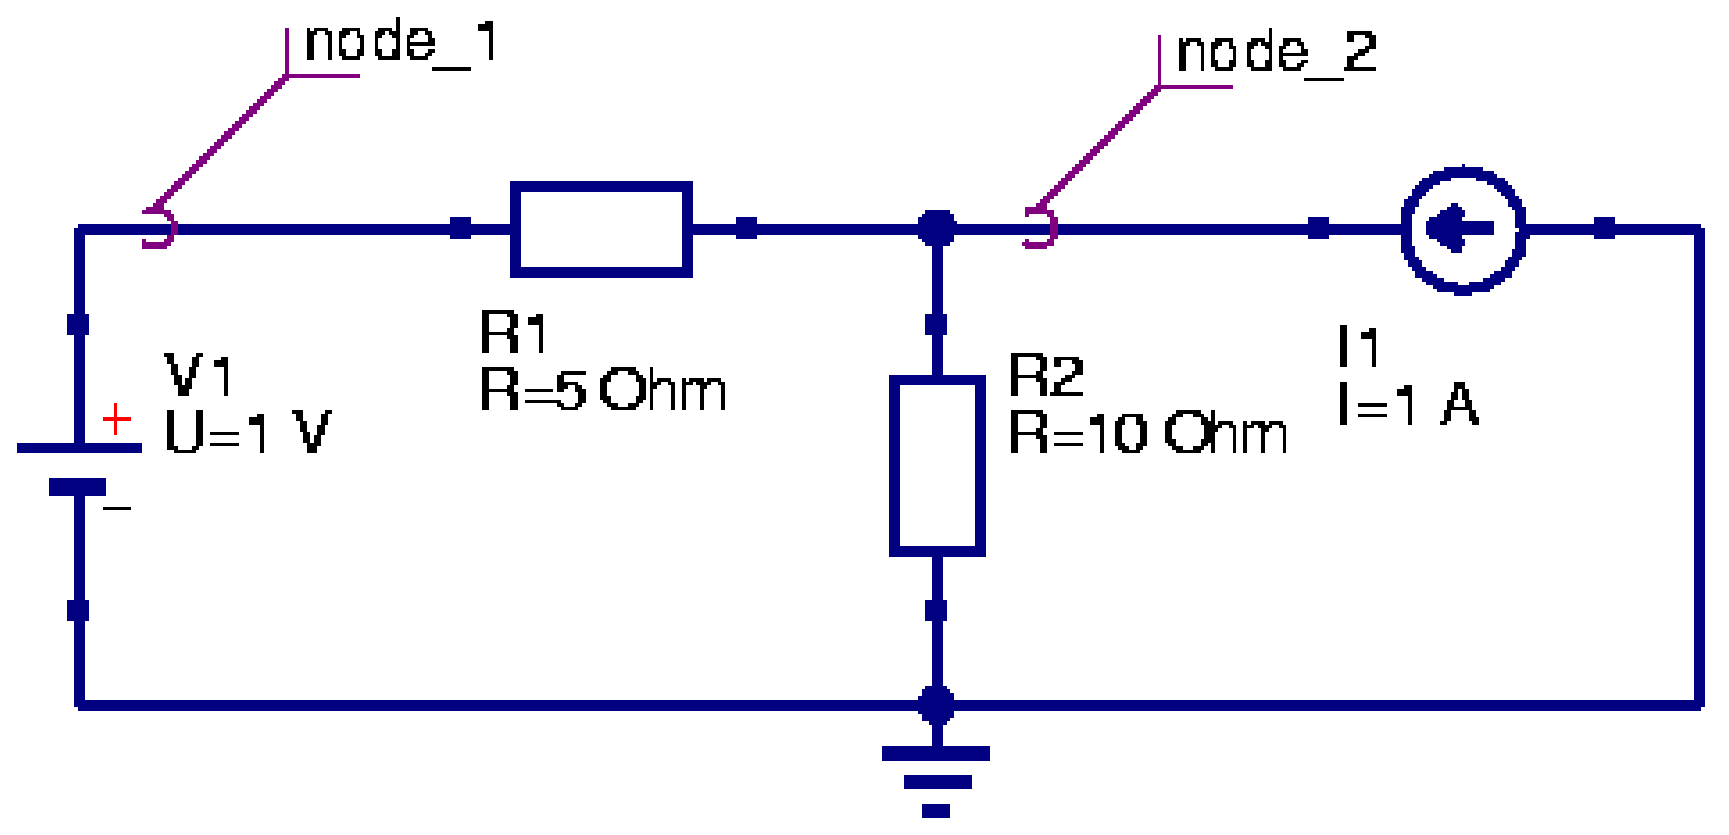
\includegraphics[angle=-90,width=10cm]{MNAexample}
\end{center}
\caption{example circuit applied to modified nodal analysis}
\label{fig:MNAexample}
\end{figure}
\FloatBarrier

\subsubsection*{Going through the MNA algorithm}
\addcontentsline{toc}{subsubsection}{Going through the MNA algorithm}

The G matrix is a 2$\times$2 matrix because there are 2 different
nodes apart from ground which is the reference node.  On the diagonal
you find the sum of the elements conductances connected to the nodes 1
and 2.  The off-diagonal matrix entries contain the negative
conductances of the elements connected between two nodes.

\begin{equation}
G =
\begin{pmatrix}
\frac{1}{R_{1}} & -\frac{1}{R_{1}}\\
-\frac{1}{R_{1}} & \frac{1}{R_{1}} + \frac{1}{R_{2}}
\end{pmatrix}
=
\begin{pmatrix}
0.2 & -0.2\\
-0.2 & 0.3
\end{pmatrix}
\end{equation}

The B matrix (which is transposed to C) is a 1$\times$2 matrix because
there is one voltage source and 2 nodes.  The positive terminal of the
voltage source $V_{1}$ is connected to node 1.  That is why

\begin{equation}
B = C^{T} =
\begin{pmatrix}
1\\
0
\end{pmatrix}
\end{equation}

and the D matrix is filled with zeros only because there are no dependent
(active and controlled) devices in the example circuit.

\begin{equation}
D =
\begin{pmatrix}
0
\end{pmatrix}
\end{equation}

The x matrix is a 1$\times$3 matrix.  The MNA equations deliver a
solution for the unknown voltages at each node in a circuit except the
reference node and the currents through each voltage source.

\begin{equation}
x =
\begin{pmatrix}
v_{1}\\
v_{2}\\
i_{V_{1}}
\end{pmatrix}
\end{equation}

The z matrix is according to the rules for building it a 1$\times$3
matrix.  The upper two entries are the sums of the currents flowing
into node 1 and node 2.  The lower entry is the voltage value of the
voltage source $V_{1}$.

\begin{equation}
z =
\begin{pmatrix}
0\\
I_{1}\\
U_{1}
\end{pmatrix}
=
\begin{pmatrix}
0\\
1\\
1
\end{pmatrix}
\end{equation}

According to the MNA algorithm the equation system is represented by

\begin{equation}
\left[A\right] \cdot \left[x\right] = \left[z\right]
\end{equation}

which is eqivalent to

\begin{equation}
\begin{pmatrix}
G & B\\
C & D
\end{pmatrix}
\cdot
\begin{pmatrix}
x
\end{pmatrix}
=
\begin{pmatrix}
z
\end{pmatrix}
\label{eq:MNAexample}
\end{equation}

In the example eq. (\ref{eq:MNAexample}) expands to:

\begin{equation}
\begin{pmatrix}
\frac{1}{R_{1}} & -\frac{1}{R_{1}} & 1\\
-\frac{1}{R_{1}} & \frac{1}{R_{1}} + \frac{1}{R_{2}} & 0\\
1 & 0 & 0
\end{pmatrix}
\cdot
\begin{pmatrix}
v_{1}\\
v_{2}\\
i_{V_{1}}
\end{pmatrix}
=
\begin{pmatrix}
0\\
I_{1}\\
U_{1}
\end{pmatrix}
\label{eq:MNAfull}
\end{equation}

The equation systems to be solved is now defined by the following
matrix representation.

\begin{equation}
\begin{pmatrix}
0.2 & -0.2 & 1\\
-0.2 & 0.3 & 0\\
1 & 0 & 0
\end{pmatrix}
\cdot
\begin{pmatrix}
v_{1}\\
v_{2}\\
i_{V_{1}}
\end{pmatrix}
=
\begin{pmatrix}
0\\
1\\
1
\end{pmatrix}
\end{equation}

Using matrix inversion the solution vector x writes as follows:

\begin{equation}
\left[x\right] = 
\left[A\right]^{-1}\cdot \left[z\right] = 
\begin{pmatrix}
v_{1}\\
v_{2}\\
i_{V_{1}}
\end{pmatrix}
=
\begin{pmatrix}
1\\
4\\
0.6
\end{pmatrix}
\label{eq:MNAresult}
\end{equation}

The result in eq. (\ref{eq:MNAresult}) denotes the current through the
voltage source $V_{1}$ is $0.6\ampere$, the voltage at node 1 is
$1\volt$ and the voltage at node 2 is $4\volt$.

\subsubsection*{How the algorithm relates to basic equations in circuit analysis}
\addcontentsline{toc}{subsubsection}{How the algorithm relates to basic equations in circuit analysis}

Expanding the matrix representation in eq. (\ref{eq:MNAfull}) to a set
of equations denotes the follwing equation system consisting of 3 of
them.

\begin{align}
\rm{I:}& \qquad 0 = \frac{1}{R_{1}}\cdot v_{1} - \frac{1}{R_{1}}\cdot v_{2} + i_{V_{1}}& \text{KCL at node 1}\\
\rm{II:}& \qquad I_{1} = -\frac{1}{R_{1}}\cdot v_{1} + \left(\frac{1}{R_{1}} + \frac{1}{R_{2}}\right)\cdot v_{2}& \text{KCL at node 2}\\
\rm{III:}& \qquad U_{1} = v_{1}& \text{constitutive equation}
\end{align}

Apparently eq. I and eq. II conform to Kirchhoff's current law at the
nodes 1 and 2.  The last equation is just the constitutive equation
for the voltage source $V_{1}$.  There are three unknowns ($v_{1}$,
$v_{2}$ and $i_{V_{1}}$) and three equations, thus the system should
be solvable.

\addvspace{12pt}

Equation III indicates the voltage at node 1 is $1\volt$.  Applying
this result to eq. II and transposing it to $v_{2}$ (the voltage at
node 2) gives

\begin{equation}
v_{2} = \frac{I_{1} + \frac{1}{R_{1}}\cdot U_{1}}{\frac{1}{R_{1}} + \frac{1}{R_{2}}} = 4\volt
\end{equation}

The missing current through the voltage source $V_{1}$ can be computed
using both the results $v_{2} = 4\volt$ and $v_{1} = 1\volt$ by
transforming equation I.

\begin{equation}
i_{V_{1}} = \frac{1}{R_{1}}\cdot v_{2} - \frac{1}{R_{1}}\cdot v_{1} = 0.6\ampere
\end{equation}

The small example, shown in fig (\ref{fig:MNAexample}), and the
excursus into artless math verifies that the MNA algorithm and classic
electrical handiwork tend to produce the same results.

\section*{Extensions to the MNA}
\addcontentsline{toc}{section}{Extensions to the MNA}

As noted in the previous sections the D matrix is zero and the B and C
matrices are transposed each other and filled with either 1, -1 or 0
provided that there are no dependent sources within the circuit.  This
changes when introducing active (and controlled) elements.

\subsection*{Voltage controlled current source}
\addcontentsline{toc}{subsection}{Voltage controlled current source}

The voltage-dependent current source (VCCS), as shown in fig.
\ref{fig:vccs}, is determined by the following equation which
introduces one more unknown in the MNA matrix.

\begin{figure}[ht]
\begin{center}
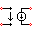
\includegraphics[width=4cm]{vccs}
\end{center}
\caption{voltage controlled current source}
\label{fig:vccs}
\end{figure}
\FloatBarrier

\begin{equation}
I_{out} = G\cdot\left(V_{1} - V_{2}\right)
\quad \rightarrow \quad
V_{1} - V_{4} - \frac{1}{G}\cdot I_{out} = 0
\label{eq:vccs}
\end{equation}

The new unknown variable $I_{out}$ must be considered by the four
remaining simple equations.

\begin{equation}
I_{1} = 0 \quad I_{2} = I_{out} \quad I_{3} = -I_{out} \quad I_{4} = 0
\end{equation}

And in matrix representation this is:
\begin{equation}
\begin{pmatrix}
.&.&.&.& 0\\
.&.&.&.& 1\\
.&.&.&.& -1\\
.&.&.&.& 0\\
1 & 0 & 0 & -1 & -\frac{1}{G}
\end{pmatrix}
\cdot
\begin{pmatrix}
V_{1}\\
V_{2}\\
V_{3}\\
V_{4}\\
I_{out}\\
\end{pmatrix}
=
\begin{pmatrix}
I_{1}\\
I_{2}\\
I_{3}\\
I_{4}\\
0\\
\end{pmatrix}
\end{equation}

As you can see the last row which has been added by the VCCS
represents the determining equation (\ref{eq:vccs}).  The additional
right hand column in the matrix keeps the system consistent.

\subsection*{Voltage controlled voltage source}
\addcontentsline{toc}{subsection}{Voltage controlled voltage source}

The voltage-dependent voltage source (VCVS), as shown in fig.
\ref{fig:vcvs}, is determined by the following equation which
introduces one more unknown in the MNA matrix.

\begin{figure}[ht]
\begin{center}
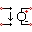
\includegraphics[width=4cm]{vcvs}
\end{center}
\caption{voltage controlled voltage source}
\label{fig:vcvs}
\end{figure}
\FloatBarrier

\begin{equation}
V_{2} - V_{3} = G\cdot \left(V_{1} - V_{4}\right)
\quad \rightarrow \quad
V_{1}\cdot G - V_{2} + V_{3} - V_{4}\cdot G = 0
\label{eq:vcvs}
\end{equation}

The new unknown variable $I_{out}$ must be considered by the four
remaining simple equations.

\begin{equation}
I_{1} = 0 \quad I_{2} = -I_{out} \quad I_{3} = I_{out} \quad I_{4} = 0
\end{equation}

And in matrix representation this is:
\begin{equation}
\begin{pmatrix}
.&.&.&.& 0\\
.&.&.&.& -1\\
.&.&.&.& 1\\
.&.&.&.& 0\\
G & -1 & 1 & -G & 0
\end{pmatrix}
\cdot
\begin{pmatrix}
V_{1}\\
V_{2}\\
V_{3}\\
V_{4}\\
I_{out}\\
\end{pmatrix}
=
\begin{pmatrix}
I_{1}\\
I_{2}\\
I_{3}\\
I_{4}\\
0\\
\end{pmatrix}
\end{equation}

\subsection*{Current controlled current source}
\addcontentsline{toc}{subsection}{Current controlled current source}

The current-dependent current source (CCCS), as shown in fig.
\ref{fig:cccs}, is determined by the following equation which
introduces one more unknown in the MNA matrix.

\begin{figure}[ht]
\begin{center}
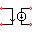
\includegraphics[width=4cm]{cccs}
\end{center}
\caption{current controlled current source}
\label{fig:cccs}
\end{figure}
\FloatBarrier

\begin{equation}
V_{1} - V_{4} = 0
\label{eq:cccs}
\end{equation}

The new unknown variable $I_{out}$ must be considered by the four
remaining simple equations.

\begin{equation}
I_{1} = -\frac{1}{G}\cdot I_{out} \quad I_{2} = I_{out} \quad I_{3} = -I_{out} \quad I_{4} = \frac{1}{G}\cdot I_{out}
\end{equation}

And in matrix representation this is:
\begin{equation}
\begin{pmatrix}
.&.&.&.& -\frac{1}{G}\\
.&.&.&.& 1\\
.&.&.&.& -1\\
.&.&.&.& \frac{1}{G}\\
1 & 0 & 0 & -1 & 0
\end{pmatrix}
\cdot
\begin{pmatrix}
V_{1}\\
V_{2}\\
V_{3}\\
V_{4}\\
I_{out}\\
\end{pmatrix}
=
\begin{pmatrix}
I_{1}\\
I_{2}\\
I_{3}\\
I_{4}\\
0\\
\end{pmatrix}
\end{equation}

\subsection*{Current controlled voltage source}
\addcontentsline{toc}{subsection}{Current controlled voltage source}

The current-dependent voltage source (CCVS), as shown in fig.
\ref{fig:ccvs}, is determined by the following equations which
introduce two more unknowns in the MNA matrix.

\begin{figure}[ht]
\begin{center}
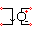
\includegraphics[width=4cm]{ccvs}
\end{center}
\caption{current controlled voltage source}
\label{fig:ccvs}
\end{figure}
\FloatBarrier

\begin{equation}
V_{1} - V_{4} = 0
\end{equation}
\begin{equation}
V_{2} - V_{3} = G\cdot I_{in}
\quad \rightarrow \quad
V_{2} - V_{3} - I_{in}\cdot G = 0
\label{eq:ccvs}
\end{equation}

The new unknown variables $I_{out}$ and $I_{in}$ must be considered by
the four remaining simple equations.

\begin{equation}
I_{1} = -I_{in} \quad I_{2} = -I_{out} \quad I_{3} = I_{out} \quad I_{4} = I_{in}
\end{equation}

The matrix representation needs to be augmented by two more new rows
(for the new unknown variables) and their corresponding columns.
\begin{equation}
\begin{pmatrix}
.&.&.&.& -1 & 0\\
.&.&.&.& 0 & -1\\
.&.&.&.& 0 & 1\\
.&.&.&.& 1 & 0\\
0 & 1 & -1 & 0 & -G & 0\\
1 & 0 & 0 & -1 & 0 & 0
\end{pmatrix}
\cdot
\begin{pmatrix}
V_{1}\\
V_{2}\\
V_{3}\\
V_{4}\\
I_{in}\\
I_{out}
\end{pmatrix}
=
\begin{pmatrix}
I_{1}\\
I_{2}\\
I_{3}\\
I_{4}\\
0\\
0
\end{pmatrix}
\end{equation}

\subsection*{Operational amplifier}
\addcontentsline{toc}{subsection}{Operational amplifier}

The ideal operational amplifier, as shown in fig.  \ref{fig:opamp}, is
determined by the following equation which introduces one more unknown
in the MNA matrix.

\begin{figure}[ht]
\begin{center}
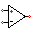
\includegraphics[width=4cm]{opamp}
\end{center}
\caption{ideal operational amplifier}
\label{fig:opamp}
\end{figure}
\FloatBarrier

\begin{equation}
V_{1} - V_{3} = 0
\label{eq:opamp}
\end{equation}

The new unknown variable $I_{out}$ must be considered by the three
remaining simple equations.

\begin{equation}
I_{1} = 0 \quad I_{2} = -I_{out} \quad I_{3} = 0
\end{equation}

And in matrix representation this is:
\begin{equation}
\begin{pmatrix}
.&.&.& 0\\
.&.&.& -1\\
.&.&.& 0\\
-1 & 0 & -1 & 0
\end{pmatrix}
\cdot
\begin{pmatrix}
V_{1}\\
V_{2}\\
V_{3}\\
I_{out}
\end{pmatrix}
=
\begin{pmatrix}
I_{1}\\
I_{2}\\
I_{3}\\
0
\end{pmatrix}
\end{equation}

The operational amplifier could be considered as a special case of a
voltage controlled current source with infinite forward
transconductance $G$.

\subsection*{Transformer}
\addcontentsline{toc}{subsection}{Transformer}

The two winding ideal transformer, as shown in fig.
\ref{fig:actrafo}, is determined by the following equation which
introduces one more unknown in the MNA matrix.

\begin{figure}[ht]
\begin{center}
\includegraphics[width=4cm]{actrafo}
\end{center}
\caption{ideal two winding transformer}
\label{fig:actrafo}
\end{figure}
\FloatBarrier

\begin{equation}
V_{2} - V_{3} = T\cdot\left(V_{1} -V_{4}\right)
\quad \rightarrow \quad
T\cdot V_{1} - V_{2} + V_{3} - T\cdot V_{4} = 0
\label{eq:trafo}
\end{equation}

The new unknown variable $I_{t}$ must be considered by the four
remaining simple equations.

\begin{equation}
I_{1} = T\cdot I_{t} \quad I_{2} = -I_{t} \quad I_{3} = +I_{t} \quad I_{4} = -T\cdot I_{t}
\end{equation}

And in matrix representation this is:
\begin{equation}
\begin{pmatrix}
.&.&.&.& T\\
.&.&.&.& -1\\
.&.&.&.& 1\\
.&.&.&.& -T\\
T & -1 & 1 & -T & 0
\end{pmatrix}
\cdot
\begin{pmatrix}
V_{1}\\
V_{2}\\
V_{3}\\
V_{4}\\
I_{t}
\end{pmatrix}
=
\begin{pmatrix}
I_{1}\\
I_{2}\\
I_{3}\\
I_{4}\\
0
\end{pmatrix}
\end{equation}

It is noticable that the additional row (part of the C matrix) and the
corresponding column (part of the B matrix) are transposed to each
other.  When considering the turns ratio $T$ being complex introducing
an additional phase the transformer can be used as phase-shifting
transformer.  Both the vectors must be conjugated complex transposed
in this case.

\subsection*{Symmetrical transformer}
\addcontentsline{toc}{subsection}{Symmetrical transformer}

The ideal symmetrical tranformator, as shown in fig.
\ref{fig:acstrafo}, is determined by the following equations which
introduce one more unknown in the MNA matrix.

\begin{figure}[ht]
\begin{center}
\includegraphics[width=4cm]{acstrafo}
\end{center}
\caption{ideal three winding transformer}
\label{fig:acstrafo}
\end{figure}
\FloatBarrier

\begin{equation}
T_{1}\cdot\left(V_{1} - V_{6}\right) = V_{2} - V_{3}
\quad \rightarrow \quad
T_{1}\cdot V_{1} - V_{2} + V_{3} - T_{1}\cdot V_{6} = 0
\end{equation}
\begin{equation}
T_{2}\cdot\left(V_{5} - V_{4}\right) = V_{2} - V_{3}
\quad \rightarrow \quad
- V_{2} + V_{3} - T_{2}\cdot V_{4} + T_{2}\cdot V_{5} = 0
\label{eq:acstrafo}
\end{equation}

The new unknown variable $I_{t}$ must be considered by the eight
remaining simple equations.

\begin{equation}
I_{1} = T_{1}\cdot I_{t} \quad I_{2} = -I_{t} \quad I_{3} = I_{t} \quad I_{6} = -T_{1}\cdot I_{t}
\end{equation}
\begin{equation}
I_{2} = -I_{t} \quad I_{3} = +I_{t} \quad I_{4} = -T_{2}\cdot I_{t} \quad I_{5} = T_{2}\cdot I_{t}
\end{equation}

The matrix representation needs to be augmented by two more new rows
and their corresponding columns.
\begin{equation}
\begin{pmatrix}
.&.&.&.&.&.& T_{1} & 0\\
.&.&.&.&.&.& -1 & -1\\
.&.&.&.&.&.& 1 & 1\\
.&.&.&.&.&.& 0 & -T_{2}\\
.&.&.&.&.&.& 0 & T_{2}\\
.&.&.&.&.&.& -T_{1} & 0\\
T_{1} & -1 & 1 & 0 & 0 & -T_{1} & 0 & 0\\
0 & -1 & 1 & -T_{2} & T_{2} & 0 & 0 & 0
\end{pmatrix}
\cdot
\begin{pmatrix}
V_{1}\\
V_{2}\\
V_{3}\\
V_{4}\\
V_{5}\\
V_{6}\\
I_{t}\\
I_{t}
\end{pmatrix}
=
\begin{pmatrix}
I_{1}\\
I_{2}\\
I_{3}\\
I_{4}\\
I_{5}\\
I_{6}\\
0\\
0
\end{pmatrix}
\end{equation}

\subsection*{Gyrator}
\addcontentsline{toc}{subsection}{Gyrator}

The ideal gyrator, as shown in fig.  \ref{fig:gyrator}, is determined
by the following equations which introduce two more unknowns in the
MNA matrix.

\begin{figure}[ht]
\begin{center}
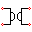
\includegraphics[width=4cm]{gyrator}
\end{center}
\caption{ideal gyrator}
\label{fig:gyrator}
\end{figure}
\FloatBarrier

\begin{equation}
I_{in} = -\frac{1}{R}\cdot\left(V_{2} - V_{3}\right)
\quad \rightarrow \quad
-\frac{1}{R}\cdot V_{2} + \frac{1}{R}\cdot V_{3} - I_{in} = 0
\end{equation}
\begin{equation}
V_{2} - V_{3} = \frac{1}{R}\cdot\left(V_{1} - V_{4}\right)
\quad \rightarrow \quad
\frac{1}{R}\cdot V_{1} - V_{2} + V_{3} - \frac{1}{R}\cdot V_{4} = 0
\label{eq:gyrator}
\end{equation}

The new unknown variables $I_{out}$ and $I_{in}$ must be considered by
the four remaining simple equations.

\begin{equation}
I_{1} = -I_{in} \quad I_{2} = -I_{out} \quad I_{3} = I_{out} \quad I_{4} = I_{in}
\end{equation}

The matrix representation needs to be augmented by two more new rows
(for the new unknown variables) and their corresponding columns.
\begin{equation}
\begin{pmatrix}
.&.&.&.& -1 & 0\\
.&.&.&.& 0 & -1\\
.&.&.&.& 0 & 1\\
.&.&.&.& 1 & 0\\
0 & -\frac{1}{R} & \frac{1}{R} & 0 & -1 & 0\\
\frac{1}{R} & -1 & 1 & -\frac{1}{R} & 0 & 0
\end{pmatrix}
\cdot
\begin{pmatrix}
V_{1}\\
V_{2}\\
V_{3}\\
V_{4}\\
I_{in}\\
I_{out}
\end{pmatrix}
=
\begin{pmatrix}
I_{1}\\
I_{2}\\
I_{3}\\
I_{4}\\
0\\
0
\end{pmatrix}
\end{equation}

\nocite{*}

\chapter*{Bibliography}
\addcontentsline{toc}{chapter}{Bibliography}
\def\chapter*{}% to suppress any header
\def\section*{}% just to be sure
\renewcommand{\bibname}{}
\bibliographystyle{IEEEtran}
\bibliography{literature}

\end{document}
